\chapter{Introduction}
In this chapter, both the concept of an emulator and the Game Boy are introduced. Furthermore, the purpose of this report, which is to develop an emulator of said console is specified.
%\section{Background}
\section{Emulators in general}
%\subsection{What is an emulator?}
An emulator generally refers to some kind of hardware or a piece of software which emulates the functionality of some other computer system \cite{emulatortechnopedia} \cite{emulatorlifewire}. While the main goal of an emulator is to imitate another computer system, an emulator may also improve upon the original system by providing additional features or by exceeding the performance of the original system \cite{emulatorlifewire}.\\
\\
Emulators are used to bridge the gap between different kinds of hardware. For example, it is possible to, within one's operating system, run other operating systems; emulate sound hardware, such as a guitar amplifier or play video games on hardware not specifically made for said games \cite{emulatorbusinessinsider}. Within the scope of this report, the term emulator refers to software used specifically to make it possible to play games on systems that are not originally intended to run these games.
\section{An Introduction to the Game Boy}
%\subsection{An Introduction to the Game Boy}
In 1989, Nintendo released the handheld video game console Game Boy, designed by the inventor Gunpei Yokoi \cite{gameboylook} \cite{gameboytimeline1}. It was the first entry in a family of video game systems, both 8-bit and 16-bit, the last of which being the Game Boy Advance Micro which was discontinued as late as 2010 \cite{gameboytimeline1}. The 8-bit Game Boy is the predecessor to Nintendo's more modern handheld consoles: the Nintendo Switch \cite{NintendoSwitch} and The Nintendo DS (Dual Screen) \cite{NintendoDSFamily} console family.\\
\\
The 1989 Game Boy, also known as DMG-01 (Dot Matrix Game), is an 8-bit handheld console characterised by its green monochromatic LCD display and bulky grey design (see Figure \ref{fig:GameBoy-fig}) \cite{gameboylook}. The other 8-bit Game Boy models are Game Boy Pocket, Game Boy Light and Game Boy Color. The Game Boy Pocket and Game Boy Light are slimmer versions of the DMG-01 with upgraded LCDs while Game Boy Color has a colour LCD and can play games not supported by the older Game Boys \cite{gameboytimeline1}. In this report Game Boy refers to either of the DMG-01, Game Boy Pocket, Game Boy Light or all of them grouped together since there are no major differences between them. The Game Boy Color and Game Boy Advance models are not covered by this report.

\begin{figure}[H]
    \centering
    \includegraphics[scale=0.3]{figures/Game-Boy-FL.png}
    \caption{The first Game Boy model, DMG-01. From \cite{gameboy-wikipedia}. Public Domain.}
    \label{fig:GameBoy-fig}
\end{figure}

The Game Boy and Game Boy Color have together sold approximately 118 million units \cite{GBSales}, making them one of Nintendo's most successful product lines ever, while also being the birthplace of popular franchises such as Kirby and Pokémon \cite{Kirby} \cite{Pokemon} \cite{gameboytimeline2}. According to Katie Smith-Wong at the entertainment news site Den of Geek \cite{gameboylook}, there are a number of factors that led to the success of the Game Boy, the first being the design of the consoles; Compared to its competitors, the Game Boy and its variations were simplistic in their design. Because of this simplicity, the Game Boy consoles were more affordable than the competing hand held consoles while also having a longer battery life. Furthermore, multiplayer mode was possible thanks to the built in game link port. This in combination with the affordability and the superior battery life made the different Game Boys excellent multiplayer consoles. The many iconic game titles also contributed to the Game Boy's success, most notably Tetris \cite{Tetris} and the Pokémon \cite{Pokemon} games, which reached out to the mainstream audience .\\
\\
Recreating the behaviour of a computer system within another computer system through software is a computationally heavy task since software is much slower than electronics; therefore, simpler computer systems were the first to be emulated on personal computers through software. During the middle of the 1990s the personal computers were powerful enough to make emulation of earlier video game consoles feasible \cite{emunation-history}. During this period Nintendo was one of the most popular media brands \cite{ask-wonder-nintendo} and thus emulators for Nintendo's consoles started to appear on the internet. The first known emulator of the Game Boy released, that could run commercial games, was an emulator by the name Virtual Game Boy. It was created by Marat Fayzullin in 1995 for some unknown system and was ported to PC somewhere between 1995 and 1996 \cite{gameboyemulationhistory}. Since then many more Game Boy emulators have been released; written in many different languages and ranging in functionality \cite{gameboyemulators}.\\
\\
The central component of the Game Boy is the DMG-CPU \cite{gameboyarchitecture} which is a chip containing a pixel processing unit (PPU), a central processing unit (CPU) and an audio processing unit (APU). Connected to the DMG-CPU are 8 KiB of RAM and video RAM (VRAM). The PPU outputs pixels, that can be one of four shades, to an LCD that is $160 \times 144$ pixels in dimensions and the audio is output either through a headphone jack or a built in speaker. Games are stored on ROM chips that come inside cartridges see Figure \ref{fig:GameBoyArch-fig}.

\begin{figure}[H]
    \centering
    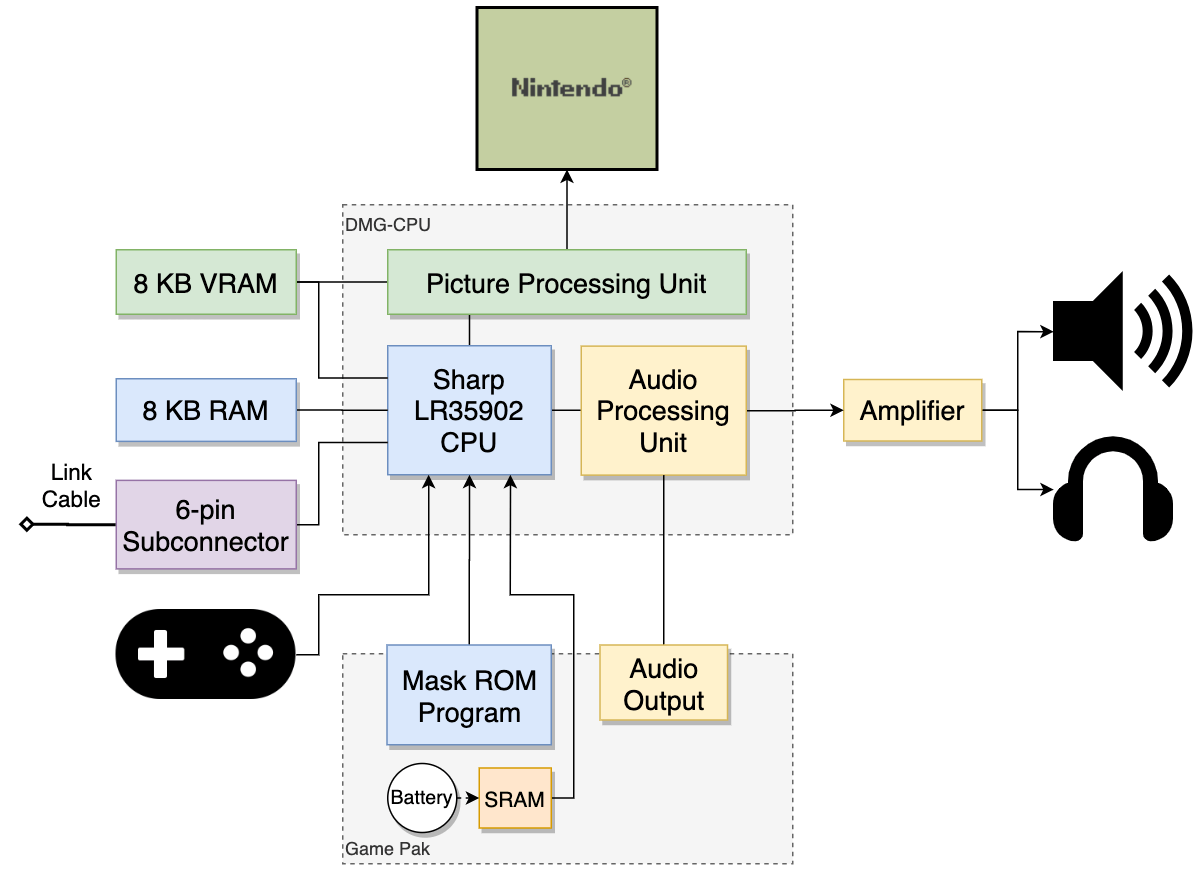
\includegraphics[scale=0.35]{figures/gbdiagram.png}
    \caption{Diagram of the architecture of the Game Boy and the general architecture of a game cartridge (Game Pak). From \cite{gameboyarchitecture}. CC BY 4.0.}
    \label{fig:GameBoyArch-fig}
\end{figure}


%; 8kb RAM; 8kb VRAM; a $160 \times 144$ pixels small LCD, which can display four shades of grey (green on the DMG-01); audio output; a game link port, used to connect multiple Game Boys; buttons for controller input and finally a slot for the game cartridges \cite{gameboyarchitecture}.


\newpage
\section{Purpose}

%The task is to program an emulator application that can read the ROM extracted from an old console game cartridge, and emulate the hardware that would run the data contained in it, displaying the graphical output the hardware would have, and providing remapped input to the user to interact with the buttons that were in the hardware, allowing them to play the game. Focus will be to have a graphical interface working, not taking sound or other systems into account. The development will suitably take place in C++. The focus is on programming the emulation for the low-level hardware.
The purpose of this thesis is to explore the possibility of developing a set of microcontrollers which can be assembled to a complete complex system. This is done through emulating the original Game Boy from 1989. As per the initial project description, focus will be on having a graphical interface working, not taking sound or other systems into account. 
\\\\
Developing an emulator presents additional purposes as a problem with older gaming consoles is that many of them are no longer produced and are therefore becoming harder and harder to come by. An emulator solves this problem by letting people play old console games on newer hardware. This thesis therefore aims to create a Game Boy emulator for the PC to allow future generations to have the same experience as the people playing the games on the original console whilst also preserving a piece of history. Additionally, the authors would like to share the accumulated knowledge of emulator development with others by providing documentation for the design as well as the code, so that others may learn from it and possibly use it as a base for their own emulators.

\section{Delimitations}
\label{sec:Delimitations}
To reduce the complexity and scope of this thesis certain delimitations have been made.
The thesis has been limited to only emulate the original Game Boy from 1989 and subsequent with equivalent hardware. This reduces the complexity of the thesis significantly as it reduces the amount of different systems and chips needed to be researched. Furthermore, it also means that the hardware which is to be researched is older and therefore of lower complexity than more modern hardware.
\\\\
Regarding some features and systems in the Game Boy, further limitations are made. First of all; ``Serial Data Transfer'' is not supported. This is a feature which is used to connect a Game Boy to another Game Boy to, amongst other things, allow for multiplayer gameplay \cite{GBWikiSerialDataTransferTutorial}. Although this could be implemented in software either by connecting two instances of the emulator on the same machine, or separate machines through internet play, this is simply not within the primary scope of emulating the Game Boy hardware. %this is simply out of scope. In the case of playing on the same machine, due to that it creates too little value for the effort, and in the case of internet play, it is no longer deemed to be within the scope of the purpose of the thesis.
%The only kind of hardware port that is regarded in this emulator is the one where you insert your games.
\\\\
The games for the Game Boy comes in cartridges called Game Paks \cite{gamepak}. The specifications of these can differ between different games with a total of 28 different configurations supported by the console, including six different memory bank controllers (MBCs) \cite{cartridgeType}. The aim is not to support all of the configurations, but rather the most significant types. 
\newpage
The Game Boy also has a feature called ``Vin'', allowing the use of external audio hardware located in the cartridge. However, none of the games made for Game Boy uses this feature \cite{pandDocsSoundControlRegisters} and is therefore excluded from being implemented in the emulator.

\section{Ethics}
\label{sec:introEthics}
Creating an emulator for a previously commercially sold product comes with complications. Because of Nintendo having created the Game Boy, it is natural that they are committed to making sure no one infringes the copyrights related to their product. When discussing emulators, there is also often a discussion of what is right and wrong, what counts as piracy and what is legal to do around the subject of copyright. 
\\\\
Nintendo Australia  states the following regarding emulators \cite{NintendoCopyright}:
\\\\
\textit{\textbf{"A Nintendo emulator is a software program that is designed to allow gameplay on a platform that it was not created for. A Nintendo emulator allows for Nintendo console based or arcade games to be played on unauthorised hardware. The video games are obtained by downloading illegally copied software, i.e. Nintendo ROMs, from Internet distributors. Nintendo ROMs then work with the Nintendo emulator to enable game play on unauthorised hardware such as a personal computer, a modified console, or another video game device."}}
\\\\
Thus, Nintendo claim that the games which are used together with emulators are obtained illegally. However, they do not explicitly state that they consider the use nor development of emulators illegal, as long as no copyrighted material is used. All of this leads to a lot of confusion around the legality and ethics of emulation, further discussion regarding this topic can be found in Section \ref{sec:Ethics}.
